\documentclass[00_mcda_tutorial.tex]{subfiles}

\begin{document}
\section*{Tutorial 1: manual data entry}
\addtocounter{section}{1}
\addcontentsline{toc}{section}{\protect\numberline{}Tutorial 1: manual data entry}

This tutorial guides you through the process of manually entering data, so that you can create your own effects tables.

\subsection*{Subjects covered}
\begin{itemize}
\item Manual data entry interface
\item Defining criteria and alternatives
\item Specifying data sources
\item Filling in the data entry table
\end{itemize}

\subsection*{Example effects table}
The data that you are going to enter in this tutorial is taken from the effects table for lixisenatide as included in the \href{https://www.ema.europa.eu/documents/template-form/day-80-assessment-report-overview-d120-loq-template-guidance-rev-0718_en.doc}{EMA Guidance document for critical assessment reports} (see page 72).  For didactic purposes, we are going to work with a simplified version of that table which includes HbA1c as a favourable effect and nausea as an unfavourable effect (Figure \ref{fig:lixisenatide_effect_table}).

\begin{figure}[!h]
    \centering
	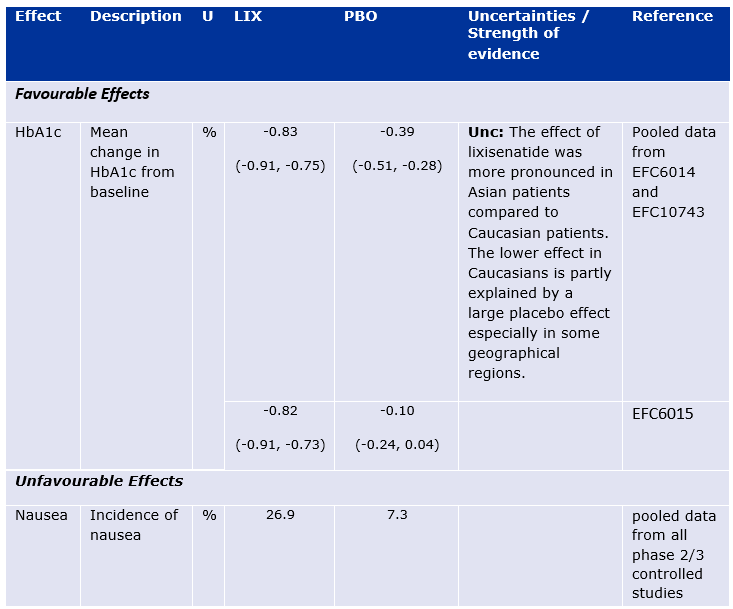
\includegraphics[width=\textwidth]{fig/lixiEffectTable.png}
    \caption{Simplified effects table for lixisenatide, a treatment for type 2 diabetes mellitus}
	\label{fig:lixisenatide_effect_table}
\end{figure}

\subsection*{Sign in to MCDA.drugis.org}
\leftpointright \, Open your browser and navigate to \href{https://mcda.drugis.org}{https://mcda.drugis.org}. Use your Google account to sign in. You will be redirected to your personal homepage, containing your previously created workspaces, both finished and unfinished (if any).

\subsection*{Create a new workspace}
\leftpointright \, Press the ‘Add workspace’ button, select the option ‘Create new workspace’, and press the ‘Add’ button. This leads to the first step of the manual entry process.
\newline

\noindent \faGraduationCap \, A workspace contains the clinical efficacy and safety data that you have entered for a particular benefit-risk assessment. Within a workspace you can build effects tables and perform quantitative benefit-risk analyses. Existing workspaces are opened by clicking on their name, or navigating to their URL directly via a link or bookmark. Workspaces can only be accessed by their owner.
\newline

\noindent \faLightbulbO \, We here cover the manual workspace creation process; besides this you can also create workspaces based on example data uploaded by the ADDIS team, and upload JSON files exported by you or another user.

\subsection*{Enter general information}
\noindent \leftpointright \, Enter a descriptive title in the ‘Workspace title’ field at the top of the page. For example, “lixisenatide data entry tutorial”. 
\newline

\noindent \leftpointright \, Enter the indication and other relevant context for your assessment in the ‘Therapeutic context’ field. For example, “Assessment of lixisenatide for the treatment of adults with type 2 diabetes mellitus to achieve glycaemic control in patients not adequately controlled on oral antidiabetics.”
\newline

\noindent \faLightbulbO \, At any stage during the data entry process you can press the ‘Save’ button at the bottom of the page to store the current state. This lets you continue later. You can navigate back to your home page by pressing the mcda.drugis.org link on the menu bar at the top-left of the screen.

\subsection*{Criteria and favorability}
\noindent \leftpointright \, The effects table for lixisenatide divides the criteria into favourable and unfavourable effects. To enable this classification, check the ‘Use favorability’ box below the ‘Criteria’ heading.
\newline

\noindent \faGraduationCap \, Criteria are the clinical efficacy and safety outcomes in terms of which the treatments under consideration are evaluated. A criterion has a name (a short identifier, such as  “HbA1c” or “Nausea”), and a description. The description specifies how the effect of a treatment on the selected outcome variable is measured statistically. For example, for “HbA1c” this could be “mean change of HbA1c from baseline” or “proportion of patients with a normal HbA1c value at week 24”.
\newline

\noindent \faGraduationCap \, For regulatory purposes, criteria can additionally be classified as favourable or unfavourable, with favourable criteria being ones where the new treatment under consideration outperforms the status quo.

\subsection*{Add the HbA1c criterion}
\noindent \leftpointright \, Click the ‘Add Criterion’ button and fill in the dialog as specified in Figure \ref{fig:crit1}.

\begin{figure}[!h]
    \centering
	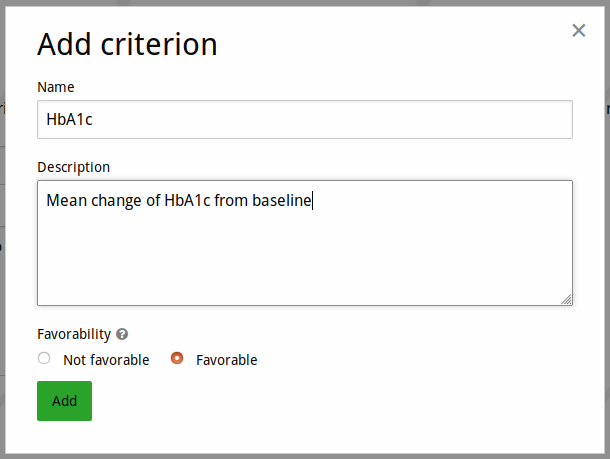
\includegraphics[width=\textwidth]{fig/addhba1c.png}
    \caption{Add criterion dialogue for HbA1c.}
	\label{fig:crit1}
\end{figure}

\subsection*{Add two data sources for HbA1c}
\noindent \faGraduationCap \, A data source is a study from which summary statistics or treatment effect estimates are taken. This can be a single pivotal study but could also be a pooled analysis, such as a combined safety pool or a (network-) meta-analysis. A data source’s origin are specified via its name (the ‘Reference’ field) and optionally its URL.
\newline

\noindent \leftpointright \, On the HbA1c criterion, click the ‘Add data source’ button. In the dialog, specify the reference “Pooled data from EFC6014 and EFC10743” and leave the ‘Reference URL’ field empty. Click the ‘Add’ button. You now should have one data source for the HbA1c criterion. Click the ‘Add data source’ button and add the second data source woth the reference “EFC6015” while leaving the ‘Reference URL’ field empty again. Then click ‘Add.’ Now there should be a second row in the data sources list for the criterion.

\subsection*{Add nausea as an unfavourable effect}
\noindent \leftpointright \, Click the ‘Add criterion’ button, fill in the dialog as specified in Figure \ref{fig:crit2}, and click ‘Add’ (note that favorability is now ‘Not favorable’).
\newline

\begin{figure}[!h]
    \centering
	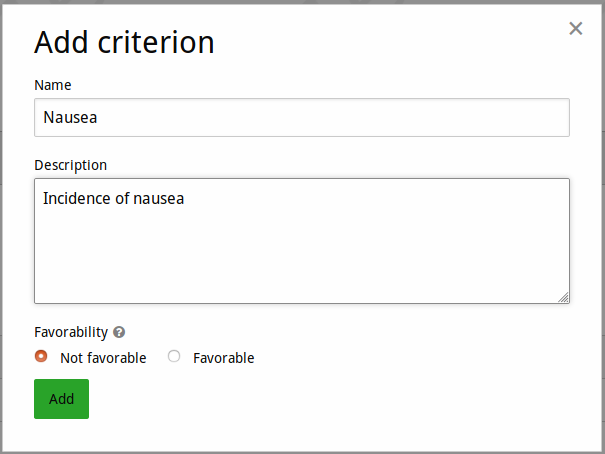
\includegraphics[width=\textwidth]{fig/addNausea.png}
    \caption{Add criterion dialog for Nausea.}
	\label{fig:crit2}
\end{figure}

\noindent \leftpointright \, Click the ‘Add data source button and enter “Pooled data from all phase 2/3 controlled studies” as the the reference for this data source.  There are no further data sources for this criterion.

\subsection*{Add lixisenatide and placebo as alternatives}
\noindent \leftpointright \, Under the ‘Alternatives’ header, click the ‘Add Alternative’ button and fill in “lixisenatide” in the ‘Title’ text box. Click the ‘Add’ button. Repeat the process and add a “placebo” alternative.

\subsection*{Proceed to data entry}
\noindent \leftpointright \, Click the ‘Enter data’ button. Take a moment to inspect the data entry table that the system has generated based on your work in the previous steps. If you spot any errors or inconsistencies, you can always click the ‘Back’ button to correct them.

\subsection*{Deterministic and SMAA tabs}
\noindent \faLightbulbO \, Data entry is split into two tabs – Deterministic and SMAA – and you can switch freely between them by clicking on the corresponding tab above the effects table. In this tutorial, we will be mainly using the ‘Deterministic’ tab.
\newline

\noindent \faGraduationCap \, Data about effects can be entered either as effects or distributions. When working with effects, the ‘Deterministic’ tab is used. Alternatively, the ‘SMAA’ tab allows the user to enter distributions to describe the effects. An overview of the various data entry possibilities is provided in the \hyperref[appendix1]{Appendix to Tutorial 1}.

\subsection*{Add a unit of measurement}
\noindent \leftpointright \, We can now add a unit of measurement for each data source. To do so, click on the edit icon in the ‘Unit of measurement’ cell.
\newline

\noindent \leftpointright \, For ‘HbA1c/Pooled data’, leave the type on ‘Custom’ and add the Label ‘\%’. Add the same unit of measurement to ‘HbA1c/EFC6015’ too.
\newline

\noindent \leftpointright \, For the Nausea data source, select ‘Proportion (percentage)’ as the unit of measurement.
\newline

\noindent \faGraduationCap \, An overview of the various units of measurement is provided in the \hyperref[appendix1]{Appendix to Tutorial 1}.

\subsection*{Add Strength of evidence/Uncertainties}
\noindent \faGraduationCap \, The ‘Uncertainties’ and ‘Strength of evidence’ fields describe any strengths and weaknesses of the study design, quality of the data collection and analysis, generalizability of the study findings, etc.
\newline

\noindent \leftpointright \, We will add the following Uncertainty to the ‘HbA1c/Pooled data’ data source: “The effect of lixisenatide was more pronounced in Asian patients compared to Caucasian patients. The lower effect in Caucasians is partly explained by a large placebo effect especially in some geographical regions.” To do so, click the edit button in the ‘Strength of evidence/Uncertainties’ cell and fill the Uncertainties text box.

\subsection*{Enter data}
\noindent \leftpointright \, Click on the ‘Missing or invalid input’ link in the HbA1c, pooled data from EFC6014 and EFC10743 row of the lixisenatide column. Fill out the dialog as shown in Figure \ref{fig:data1}, and click anywhere on the page outside of the dialog to close it.

\begin{figure}[!h]
    \centering
	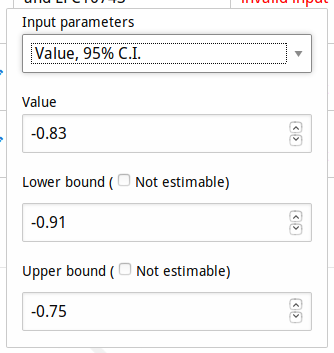
\includegraphics[width=.5\textwidth]{fig/effectsInput.png}
    \caption{Data entry dialog for HbA1c.}
	\label{fig:data1}
\end{figure}

\noindent \leftpointright \, Proceed to fill out the remaining three cells for HbA1c with the point estimates and 95\% confidence intervals from Figure \ref{fig:lixisenatide_effect_table}.
\newline

\noindent \leftpointright \, Similarly, fill out the cells for Nausea with the values from Figure \ref{fig:lixisenatide_effect_table}, selecting ‘Value’ as the input parameter. Your final data entry table should look like Figure \ref{fig:dataFinished} (‘Strength of evidence/Uncertainities’ column is omitted here to provide a better overview).

\begin{figure}[!h]
    \centering
	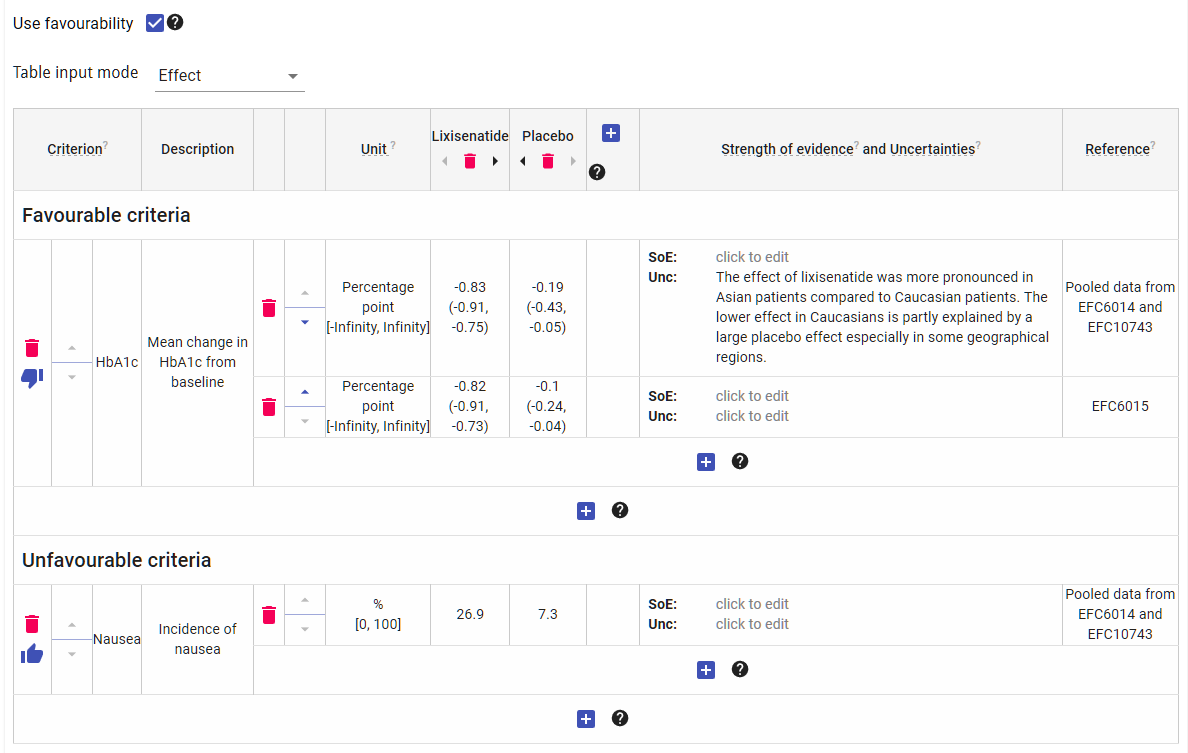
\includegraphics[width=\textwidth]{fig/effectsInputDone.png}
    \caption{Final data entry table for lixisenatide.}
	\label{fig:dataFinished}
\end{figure}

\noindent \faLightbulbO \, If required, cells can be left empty by choosing the ‘Empty cell’ as the input parameter.

\subsection*{Generate distributions}
\noindent \leftpointright \, If a user wishes to work with distributions and perform SMAA analyses but the data is provided as effects only, it is possible to automatically generate the distributions. To do so, click the ‘Generate distributions’ button. Doing this will take you to the ‘SMAA’ tab where the automatically generated data is presented. Please see the \hyperref[appendix1]{Appendix to Tutorial 1} to see which effect input types are converted into which distribution types.

\subsection*{Finalize entry}
You have now finished preparing your effects table for analysis.
\newline

\noindent \leftpointright \, Click ‘Done’ and you will go to the overview page of your newly-created workspace where you will find the entered effects table.
\newline

\noindent \faGraduationCap \, After finishing the manual entry process, cosmetic properties such as names and descriptions can still be edited, and the criteria can be re-ordered using the arrow buttons. However, to prevent breaking the analyses that are based on them, measurements cannot be modified. Changing measurements can be done by creating a copy of the workspace on your homepage. This begins a new manual entry process as detailed above, but all criteria, alternatives and measurements are already filled out based on the old workspace, and can be changed at will.

\subsection*{Export and share with others}
\noindent \leftpointright \, On your newly-created workspace, click ‘Download workspace’ in the top-left to save a .json file which contains all the data you just entered. When creating a new workspace, you can upload this file (using the ‘local file’ option) and the new workspace will contain a copy of your data.
\newline

\noindent \faLightbulbO \, Sending this file via e.g. email to someone else is the recommended way to share workspace data with other users.
\clearpage



%=========== APPENDIX =====================


\section*{Appendix to Tutorial 1: data source characteristics and data entry options}
\label{appendix1}
\addcontentsline{toc}{section}{\protect\numberline{}Appendix to Tutorial 1}

A treatment effect is a statistical parameter that describes how a given treatment affects the distribution of a criterion in the target population (i.e., all patients for which the evaluated treatment is indicated). The representation of that parameter’s uncertainty in the effects table depends on the specified characteristics of the row’s data source. Indicating that the input type is ‘Distribution’ corresponds to a Bayesian perspective, where the uncertainty is quantified by means of probability distributions. The option ‘Effect’ corresponds to a frequentist perspective where parameters are treated as fixed but unknown constants for which point and interval estimates (e.g., 95\% confidence intervals) are provided.

\subsection*{Types of distributions (Bayesian)}
Distributions can be specified directly by choosing a type of distribution and entering its parameters, or derived indirectly from summary statistics from a clinical study (option ‘Generate distributions’). When this latter option is selected, a Bayesian posterior distribution (i.e., a beta distribution for the event probability of a dichotomous outcome variable and a normal distribution for the mean of a continuous outcome variable) is estimated from the summary statistics supplied by the user and a reference prior set by the system.
\newline

\noindent The following types of distribution are supported:
\begin{itemize}
\item Beta
\item Normal
\item Gamma
\item Value (i.e., degenerate distribution that always results in the same value)
\item Range
\end{itemize}

\noindent Distributions of the type 'Value' and 'Range' can be input either as percentages, decimals, or neither, see Section \ref{sec:uom}.
    
\subsection*{Types of effects (Frequentist)}
The following data entry options are currently available for effects:
\begin{itemize}
\item Value
\item Value, 95\% confidence interval
\item Range
\end{itemize}

\noindent These effects can be input either as percentages, decimals, or neither, see Section \ref{sec:uom}.
 
\subsection*{Unit of measurement}
\label{sec:uom}
The following units of measurement are supported:
\begin{itemize}
\item Custom: you can input a custom label and any lower and upper bounds.
\item Proportion (decimal): label will be set to 'Proportion', and lower and upper bounds to 0 and 1, respectively.
\item Proportion (percentage): label will be set to '\%', and lower and upper bounds to 0 and 100, respectively.
\end{itemize}

\noindent You can switch between 'Percentages' and 'Decimals' views by changing the workspace settings (accessed by clicking the 'settings' button at the top right of the screen for any finished workspace). This will automatically scale the values were possible, i.e. datasources with either 'Proportion (decimal)' or 'Proportion (percentage)' unit of measurement.
\newline

\noindent The user can enter '\%' as a label for a custom unit of measurement  for a data source. However, switching between 'Percentages' and 'Decimals' views will not scale the values in this case.

\end{document}